The characteristic analysis carried out above is now applied to specific problems of solid mechanics. Both linear and non-linear problems which solutions involve several types are waves are considered. As we shall see, the development of exact solutions of Riemann problems highly depends on the different characteristic structure involved by linear elastic, elastoplastic and hyperelastic solids.
%% Then by specializing the results to problems involving a linear elastic bar and a hyperelastic Saint-Venant-Kirchhoff medium, we shall see that different types of waves may propagate within solids.

\subsection{Linear elastodynamics problems}
\label{subsec:charac_Linear_problems}
A homogeneous hyperbolic system of dimension $m$ is considered in a linear elastic solid so that the Riemann problem in the arbitrary direction $\vect{n}$ reads:
\begin{equation}
  \label{eq:Linear_Riemann_problem}
  \begin{aligned}
  &\Qcb_t + \drond{\Fcb\cdot \vect{n}}{x_n} = \vect{0}, \\
  &\left\lbrace 
    \begin{aligned}
      & \Qcb(x_n,t=0) = \Qcb^L \quad \text{if } x_n< 0\\
      & \Qcb(x_n,t=0) = \Qcb^R \quad \text{if } x_n> 0
    \end{aligned}
    \right.
  \end{aligned}
\end{equation}

\subsubsection*{Characteristic variables -- Waves solution}
By introducing a set of \textit{characteristic variables} $\Pcb=\Rbsf^{-1}\Qcb$ ($\Rsf_{ij}=\Rc^j_i$), the quasi-linear form of system \eqref{eq:Linear_Riemann_problem} can be rewritten:
\begin{equation*}
  \begin{aligned}
    &\drond{\Pc_i}{t} + c_i\drond{\Pc_i}{x} = 0 \\
    &\left\lbrace 
      \begin{aligned}
        & \Pc_i(x,t=0) = \Pc_i^L \quad \text{if } x< 0\\
        & \Pc_i(x,t=0) = \Pc_i^R \quad \text{if } x> 0
      \end{aligned}
    \right.
  \end{aligned}
\end{equation*}
\begin{figure}[h]
  \centering
  \subcaptionbox*{}[0.45\linewidth]{\begin{tikzpicture}[scale=0.75]
  \draw[->] (-4,0) -- (4.,0) node[right] {$x$};
  \draw[->] (0,0) -- (0,4.5) node[above] {$t$};
  \draw[thick] (0,0) -- (4.,4) node [right] {$c_i$};
  % \fill[black] (1.,3.) circle (0.05) node [above] {$P$};
  % \fill[black] (2.10,1.762499) circle (0.05) node [right] {$P'$};
  \draw[dotted] (-4,1.)-- (0,1) node [above left] {$t_1$} --(4.,1);
  \draw[dotted] (-4,2.)-- (0,2) node [above left] {$t_2$} --(4.,2);
  \node[above left] at (0,0) {$t_0$};
\end{tikzpicture}

%%% Local Variables:
%%% mode: latex
%%% TeX-master: "../../mainManuscript"
%%% End:}
  \subcaptionbox*{}[0.45\linewidth]{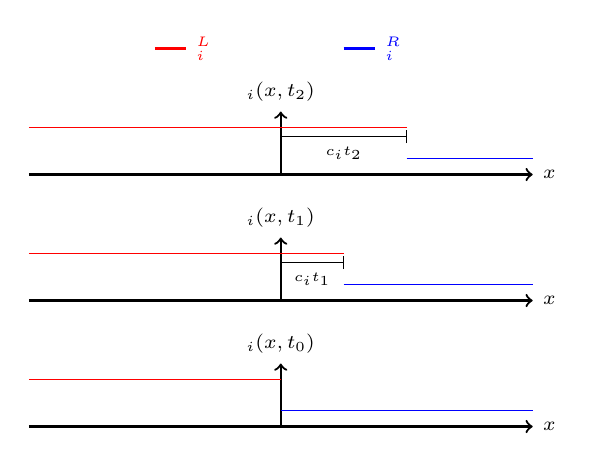
\begin{tikzpicture}[scale=0.8]
  %% t2
  \draw[->,thick] (0,0) -- (0,1) node [above] {\scriptsize$\Pc_i(x,t_2)$};
  \draw[->,thick] (-4,0) -- (4,0) node [right] {\scriptsize$x$};
  \draw[Blue] (2,0.25) -- (4,0.25);
  \draw[Red] (-4,0.75) -- (2,0.75);
  \draw (0,0.6)--(2,0.6) node [midway, below] {\tiny $c_it_2$};
  \draw (2,0.5)--(2,0.7);
  %% t1
  \draw[->,thick] (0,-2) -- (0,-1) node [above] {\scriptsize$\Pc_i(x,t_1)$};
  \draw[->,thick] (-4,-2) -- (4,-2) node [right] {\scriptsize$x$};
  \draw[Blue] (1,0.25-2) -- (4,0.25-2);
  \draw[Red] (-4,0.75-2) -- (1,0.75-2);
  \draw (0,0.6-2)--(1,0.6-2) node [midway, below] {\tiny $c_it_1$};
  \draw (1,0.5-2)--(1,0.7-2);
  %% t0
  \draw[->,thick] (0,-4) -- (0,-3) node [above] {\scriptsize$\Pc_i(x,t_0)$};
  \draw[->,thick] (-4,-4) -- (4,-4) node [right] {\scriptsize$x$};
  \draw[Blue] (0,0.25-4.) -- (4,0.25-4.);
  \draw[Red] (-4,0.75-4.) -- (0,0.75-4.);
  %% legend
  \draw[thick,Red] (-2.,2.) -- (-1.5,2.) node [right] {\scriptsize$\Pc_i^L$};
  \draw[thick,Blue] (1,2.) -- (1.5,2.) node [right] {\scriptsize$\Pc_i^R$};
\end{tikzpicture}
%%% Local Variables:
%%% mode: latex
%%% TeX-master: "../../mainManuscript"
%%% End:}
  \caption{Solution to linear advection equation on the quantity $\Pc_i$ with characteristic speed $c_i$.}
  \label{fig:advection}
\end{figure}
with $\Csf_{ij}=c_i\delta_{ij}$, the matrix of eigenvalues so that $\Jsf_{ij} \Rc^j_K = \Rc^K_i\Csf_{Kj}$. The solution of this problem is straightforward since it corresponds to a superposition of scalar linear advection equations namely, the initial profile $\Pc_i(x,t=0)$ simply propagates with speed $c_i$ as depicted in figure \ref{fig:advection}. Thus, the solution  $\Pc_i(x,t)$ at a given point is given by tracing backward the characteristic of slope $c_i$ passing through this point to the $x$-axis, that is: $\thomas{\Pc_i(x,t)=\Pc_i(x-c_it,0)}$  \cite[p.52]{Toro}. 
The vector $\Qcb$ is then determined by inverting the relation:
\begin{equation}
  \label{eq:Q_expansion}
  \Qcb(x,t) = \sum_{i=1}^m \Rcb^i \Pc_i(x-c_it,0) \quad \Rightarrow
  \left\lbrace
    \begin{aligned}
      & \Qcb(x<0,0)=\Qcb^L=\sum_{i=1}^{m}\Rcb^i \Pc_i^L\\
      & \Qcb(x>0,0)=\Qcb^R= \sum_{i=1}^{m}\Rcb^i \Pc_i^R
    \end{aligned}
    \right.
\end{equation}
Equation \eqref{eq:Q_expansion} is an eigenvector expansion with coefficients $\Pc_i^{R,L}$ from which we see that $\Qcb$ is linear a superposition of $m$ waves, each of which having the shape $\Rcb^i \Pc_i(x,0)$. Noticing that for given values of $x$ and $t$, there exists one characteristic $I$ such that $x-c_i t >0$ for all $i\leq I$, and $x-c_{I+1} t <0$ for all $i>I$, equation \eqref{eq:Q_expansion} can be rewritten \cite[p.56]{Toro}:
\begin{equation}
  \label{eq:Q_expansion_sides}
  \Qcb = \sum_{i=1}^I \Rcb^i \Pc_i^R + \sum_{i=I+1}^m \Rcb^i \Pc_i^L
\end{equation}
or, introducing the expansions of initial data \eqref{eq:Q_expansion_sides}:
\begin{align}
  &\Qcb = \sum_{i=1}^m \Rcb^i \Pc_i^R - \sum_{i=I+1}^m \Rcb^i \(\Pc_i^R - \Pc_i^L\)= \Qcb^R - \sum_{i=I+1}^m \Rcb^i \(\Pc_i^R - \Pc_i^L\) \\
  &\Qcb= \sum_{i=1}^{m}\Rcb^i \Pc_i^L + \sum_{i=1}^I \Rcb^i \(\Pc_i^R - \Pc_i^L\)= \Qcb^L + \sum_{i=1}^I \Rcb^i \(\Pc_i^R - \Pc_i^L\) 
\end{align}
Those equations are equivalent to jump conditions across multiple discontinuous waves:
\begin{align}
  \label{eq:jump_star_R}
  &  \Qcb-\Qcb^R = -\sum_{i=I+1}^{m} \Rcb^i\delta^i \\
  \label{eq:jump_star_L}
  &  \Qcb-\Qcb^L = \sum_{i=1}^{I} \Rcb^i\delta^i \\
\end{align}
where $\Qcb(x,t)$ is the state lying in the region of the ($x,t$) plane delimited by the $I$th and $(I+1)$th characteristics, and $\Rcb^i\delta^i$ the jump carried by the $i$th wave. The coefficients $\delta^i=\Pc_i^R - \Pc_i^L$ are called the \textit{wave strengths} and can be computed from the expansions of initial conditions by solving:
\begin{equation}
  \label{eq:delta_system}
  \Qcb^R-\Qcb^L=\sum_{i=1}^{m}\Rcb^i \delta^i=\Rbsf \vect{\delta}
\end{equation}

We see that the solutions of Riemann problem \eqref{eq:Linear_Riemann_problem} consist in discontinuous waves emanating from the origin of the $(x,t)$ plane. Across such discontinuous waves, the following condition is satisfied \cite{Toro}:
\begin{definition}
  The \textbf{Rankine-Hugoniot condition} is satisfied across a discontinuous wave of speed $s_i$ associated to the $i$th characteristic field, which is solution of the hyperbolic system $\Qcb_t + \Fcb(\Qcb)_x=\vect{0}$:
\begin{equation}
  \label{eq:rankine-hugoniot}
  \saut{ \Fcb} = s_i \saut{ \Qcb}
\end{equation}
where $\saut{\bullet}$ denotes the jump operator across the discontinuity. The Rankine-Hugoniot condition is also valid for shock waves that will be met for non-linear problems in section \ref{sec:SVK_solution}.
\end{definition}

\subsubsection*{Solution of the elastic bar problem}
The above discussion is now specified to a one-dimensional elastic medium of density $\rho$ undergoing one-dimensional stress and strain states within the infinitesimal framework: $\tens{\eps}=\eps\: \vect{e}_1\otimes \vect{e}_1$ ; $\tens{\sigma}=\sigma \:\vect{e}_1\otimes \vect{e}_1$. As a consequence, the bar hypothesis holds with $\vect{v}=v \vect{e}_1$. Neglecting body forces and introducing \textit{Young's modulus E} such that $\sigma = E\eps$, the Riemann problem takes the form \eqref{eq:Linear_Riemann_problem} with conserved quantities and flux vector:
\begin{equation*}
  \Qcb = \matrice{v \\ \sigma} \quad ; \quad \Fcb = \matrice{-\frac{1}{\rho}\sigma \\ -Ev}
\end{equation*}
where $v=\vect{v}\cdot{e}_1$. The eigenvalues and left eigenvectors of the corresponding Jacobian matrix are:
\begin{equation*}
  \left\lbrace
    \begin{aligned}
      & c_1=- \sqrt{\frac{E}{\rho} }=-c\\
      & c_2= \sqrt{\frac{E}{\rho} }=c
    \end{aligned}\right.
 \quad ; \quad \Lcb^p=\[\rho c_p \:,\: -1\] \quad ; \quad \Rcb^p=\matrice{1\\- \rho c_p } 
\end{equation*}
The characteristic structure of the solution consisting of two elastic discontinuities emanating from the origin of the ($x,t$) plane is depicted in figure \ref{fig:elasticity_example}.
\begin{figure}[h]
  \centering
  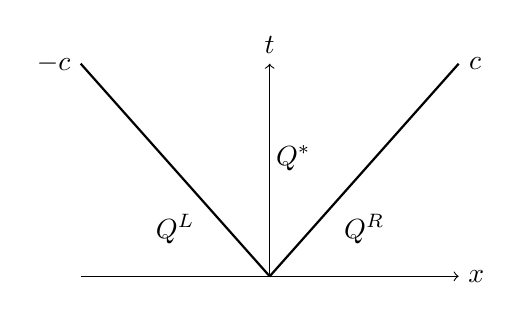
\begin{tikzpicture}[scale=0.6]
  \draw[->] (-4,0) -- (4.,0) node[right] {$x$};
  \draw[->] (0,0) -- (0,4.5) node[above] {$t$};
  \draw[thick] (0,0) -- (4.,4.5) node [right] {$c$};
  \draw[thick] (0,0) -- (-4.,4.5) node [left] {$-c$};
  \node at (2.,1.) {$\vect{Q}^R$};
  \node at (-2.,1.) {$\vect{Q}^L$};
  \node at (0.5,2.5) {$\vect{Q}^*$};
\end{tikzpicture}



%%% Local Variables:
%%% mode: latex
%%% TeX-master: "../../mainManuscript"
%%% End:

  \caption{Solution to Riemann problem \eqref{eq:Linear_Riemann_problem} for an elastic bar.}
  \label{fig:elasticity_example}
\end{figure}
The solution $\Qcb^*$ lying in the region bounded by the two elastic waves is computed by means of equation \eqref{eq:jump_star_L} after solving \eqref{eq:delta_system} for the wave strength coefficients. For a system of dimension $2$ by writing $\Qcb^R-\Qcb^L=\Delta \Qcb$ those wave strengths read:
%For a system of dimension $2$, the solution in terms of wave strengths coefficients of system \eqref{eq:delta_system} is, by writing $\Qcb^R-\Qcb^L=\Delta \Qcb$:
%Writing $\Qcb^R-\Qcb^L=\Delta \Qcb$, linear systems of dimension $2$ lead to wave strengths coefficients:
\begin{equation}
  \label{eq:wave_strengths}
  \vect{\delta} = \frac{1}{\Rc^1_1\Rc^2_2 -\Rc_1^2\Rc^1_2}\matrice{\Rc^2_2\Delta \Qc_1 - \Rc^2_1\Delta \Qc_2 \\ \Rc^1_1\Delta \Qc_2 - \Rc_2^1\Delta \Qc_1}
\end{equation}
and more specifically for a bar:
\begin{equation}
  \label{eq:wave_strengths_bar}
  \vect{\delta} = \frac{1}{2\rho c}\matrice{\rho c \Delta v + \Delta \sigma \\  \rho c \Delta v -\Delta \sigma }
\end{equation}
Hence, equation \eqref{eq:jump_star_L} yields the solution:
\begin{equation}
  \label{eq:solution_charac_variables}
  \Qcb^* = \Qcb^L +\Rcb^1 \delta^1 = \matrice{\frac{\sigma_R - \sigma_L}{2\rho c} + \frac{v_R+v_L}{2} \\ \rho c\frac{v_R - v_L}{2} + \frac{\sigma_R+\sigma_L}{2}} 
\end{equation}


\subsection{Elastic-plastic media in the geometrical linearized limit}
\label{subsec:elasto-plastic_problem}
We now consider a homogeneous one-dimensional elastoplastic medium, $x\in\[-l,l\]$, under the bar assumption. The bar is made of a linear hardening material of mass density $\rho$, tensile yield stress $\sigma^y$ and Young's modulus $E$, under the bar assumption. For such a solid domain, the Riemann problem \eqref{eq:Linear_Riemann_problem} can be written by means of the following conserved quantities and flux vectors \cite{Thomas_EP}:
\begin{equation*}
  \Qcb = \matrice{v \\ \sigma} \quad ; \quad \Fcb = \matrice{-\frac{1}{\rho}\sigma \\ -Hv}
\end{equation*}
where $H=E$ for elastic loadings while $H=d\sigma/d\eps$ is the tangent modulus for elastic-plastic evolutions. In addition, Riemann-type data on the horizontal velocity (\textit{i.e. }$v(x<0,0)=v_L\:;\:v(x>0,0)=v_R$) are used as initial conditions, so that plastic flow may occur.

%We now generalize the previous discussion to elastoplastic solids within the small strains framework. A plane wave problem in an infinite elastoplastic medium with linear hardening is then considered. Such a plane wave can be due for instance to Riemann-type data on the horizontal velocity (\textit{i.e. }$v(x<0,0)=v_L\:;\:v(x>0,0)=v_R$) so that plastic flow may occur.
% The exact solution of such a linear problem being known \cite{Wang} an exact Riemann solver, which however requires a particular procedure, may be used.
The discontinuity of $H$ across the plastic threshold prevents here the direct derivation of the solution by using the above approach. Indeed, two sets of characteristic speeds and associated eigenvectors must be considered, that is \cite{Thomas_EP,Wang}:
\begin{equation*}
  c=\pm\sqrt{\frac{H}{\rho} } \quad ; \quad \Lcb^p=\[\rho c_p \:,\: -1\] \quad ; \quad \Rcb^p=\matrice{1\\- \rho c_p } 
\end{equation*}
Waves are referred to as elastic waves for $H=E$ and as plastic ones when $H=d\sigma/d\eps$. Whether a plastic wave appears or not hence depends on the tangent modulus and subsequently, on the yield function. A prediction-correction procedure must thus be followed by first solving an elastic Riemann problem which resulting (trial) solution $\Qcb$ is tested against the yield criterion on both sides $x<0$ or $x>0$. With possibly different yield stresses, plastic strains and hardening parameters in left and right regions, the yield criterion may be violated or not, leading to one, two or no plastic wave that must be added as a correction to the original problem. Figure \ref{fig:EP_bar_solution}\subref{subfig:ep_bar_charac_4waves} shows a solution involving two plastic waves and figure \ref{fig:EP_bar_solution}\subref{subfig:ep_bar_stress_4waves}, the corresponding stress field in the bar.

\begin{figure}[h!]
  \centering
  \subcaptionbox{Characteristic structure\label{subfig:ep_bar_charac_4waves}}{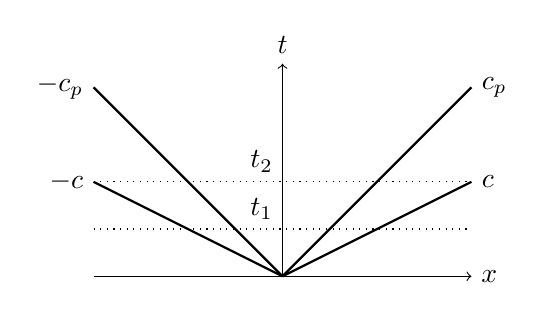
\begin{tikzpicture}[scale=0.6]
  \draw[->] (-4,0) -- (4.,0) node[right] {$x$};
  \draw[->] (0,0) -- (0,4.5) node[above] {$t$};
  \draw[thick] (0,0) -- (4.,2) node [right] {$c$};
  \draw[thick] (0,0) -- (4.,4) node [right] {$c_p$};
  \draw[thick] (0,0) -- (-4.,2) node [left] {$-c$};
  \draw[thick] (0,0) -- (-4.,4) node [left] {$-c_p$};
  \draw[dotted] (-4,1.)-- (0,1) node [above left] {$t_1$} --(4.,1);
  \draw[dotted] (-4,2.)-- (0,2) node [above left] {$t_2$} --(4.,2);
\end{tikzpicture}

%%% Local Variables:
%%% mode: latex
%%% TeX-master: "../../mainManuscript"
%%% End:}
  \subcaptionbox{Stress profile in the bar\label{subfig:ep_bar_stress_4waves}}{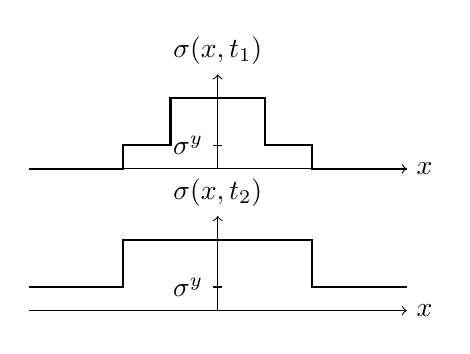
\begin{tikzpicture}[scale=0.6]
\draw[->] (0,0) -- (0,2) node [above] {$\sigma(x,t_1)$};
\draw[->] (-4,0) -- (4,0) node [right] {$x$};
\draw[thick] (-4,0) --(-2,0) -- (-2,0.5) -- (-1,0.5) -- (-1,1.5) -- (1,1.5) -- (1,0.5) -- (2,0.5) -- (2,0) -- (4,.0);
\draw (-0.1,0.5) node[left] {$\sigma^y$}-- (0.1,0.5);

\draw[->] (0,0-3) -- (0,2-3) node [above] {$\sigma(x,t_2)$};
\draw[->] (-4,0-3) -- (4,0-3) node [right] {$x$};
\draw[thick] (-4,0.5-3)  -- (-2,0.5-3)  --(-2,1.5-3) -- (2,1.5-3) -- (2,.5-3) -- (4,.5-3);
\draw (-0.1,0.5-3) node[left] {$\sigma^y$}-- (0.1,0.5-3);

\end{tikzpicture}}
  % \\\subcaptionbox{3-waves solution ($\sigma_L^y>\sigma_R^y$)\label{subfig:ep_bar_charac_3waves}}{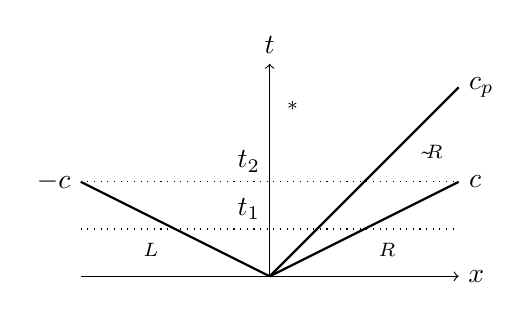
\begin{tikzpicture}[scale=0.6]
  \draw[->] (-4,0) -- (4.,0) node[right] {$x$};
  \draw[->] (0,0) -- (0,4.5) node[above] {$t$};
  \draw[thick] (0,0) -- (4.,2) node [right] {$c$};
  \draw[thick] (0,0) -- (4.,4) node [right] {$c_p$};
  \draw[thick] (0,0) -- (-4.,2) node [left] {$-c$};
  %\draw[thick] (0,0) -- (-4.,4) node [left] {$-c_p$};
  \draw[dotted] (-4,1.)-- (0,1) node [above left] {$t_1$} --(4.,1);
  \draw[dotted] (-4,2.)-- (0,2) node [above left] {$t_2$} --(4.,2);
  \node at (-2.5,0.) [above]{$\Qcb^L$};
  \node at (+2.5,0.) [above] {$\Qcb^R$};
  %\node at (-3.5,2.5) {$\tilde{\Qcb}^L$};
  \node at (+3.5,2.5) {$\tilde{\Qcb}^R$};
  \node at (0.5,3.5)  {$\Qcb^*$};
\end{tikzpicture}

%%% Local Variables:
%%% mode: latex
%%% TeX-master: "../../mainManuscript"
%%% End:}
  % \subcaptionbox{Stress for 3-waves($\sigma_L^y>\sigma_R^y$)\label{subfig:ep_bar_stress_3waves}}{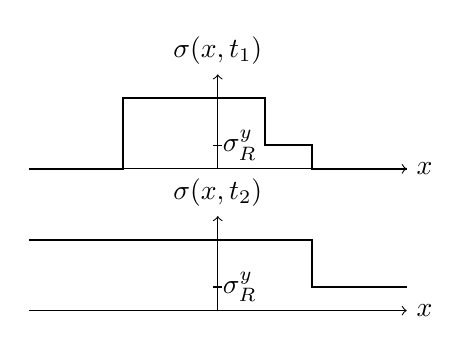
\begin{tikzpicture}[scale=0.6]
\draw[->] (0,0) -- (0,2) node [above] {$\sigma(x,t_1)$};
\draw[->] (-4,0) -- (4,0) node [right] {$x$};
\draw[thick] (-4,0) --(-2,0) -- (-2,1.5) -- (-0,1.5) -- (-0,1.5) -- (1,1.5) -- (1,0.5) -- (2,0.5) -- (2,0) -- (4,.0);
\draw (-0.1,0.5) node[right] {$\sigma_R^y$}-- (0.1,0.5);

\draw[->] (0,0-3) -- (0,2-3) node [above] {$\sigma(x,t_2)$};
\draw[->] (-4,0-3) -- (4,0-3) node [right] {$x$};
\draw[thick] (-4,1.5-3)  -- (-0,1.5-3)  --(-0,1.5-3) -- (2,1.5-3) -- (2,.5-3) -- (4,.5-3);
\draw (-0.1,0.5-3) node[right] {$\sigma_R^y$}-- (0.1,0.5-3);

\end{tikzpicture}}
  \caption{Examples of solution of Riemann problem in a homogeneous elastoplastic bar with linear hardening and initial plastic strain $\eps^p(x,0)= 0$.}
  \label{fig:EP_bar_solution}
\end{figure}
If neither $f_L$ nor $f_R$ leads to a violation of the criterion, the problem is elastic and the trial state is the solution. Otherwise, the plastic correction is performed by computing the stress in regions of the ($x,t$) plane bounded by elastic and plastic waves ($\tilde{\Qcb}^{L,R}$ in figure \ref{fig:EP_bar_solution}\subref{subfig:ep_bar_charac_4waves}) so that the yield function satisfies $f_{L,R}=0$. Then, the velocity and elastic wave strengths in yielding regions are given by solving:
\begin{align}
  & \tilde{\Qcb}^R = \Qcb^R - \delta^1_E \Rcb^1_E\\
  & \tilde{\Qcb}^L = \Qcb^L + \delta^2_E \Rcb^2_E
\end{align}
At last a plastic Riemann solver leading to the solution of the problem $\Qcb^*$ by solving successively system \eqref{eq:delta_system} for plastic wave strengths and either system \eqref{eq:jump_star_R} or \eqref{eq:jump_star_L}, that is:
\begin{equation}
  \label{eq:plastic_approx_RS}
  \vect{\delta}_P = \Rbsf^{-1}\(\tilde{\Qcb}^R- \tilde{\Qcb}^L\) \quad \Rightarrow \quad
  \Qcb^* = \left\lbrace
  \begin{aligned}
      &  \tilde{\Qcb}^R - \delta_P^2 \Rcb^2_P\\
      &  \tilde{\Qcb}^L + \delta_P^1 \Rcb^1_P
  \end{aligned}
  \right.
\end{equation}

% \begin{remark}
%   Note that the above solver also applies to bar problems characterized by stress and strain such that $\tens{\sigma}=\sigma \vect{e}_1\otimes \vect{e}_1$ ; $\tens{\eps}=\eps \vect{e}_1\otimes \vect{e}_1$, and different wave speeds.
% \end{remark}


\subsection{Hyperelastic media: A Saint-Venant-Kirchhoff solution}
\label{sec:SVK_solution}
The approaches followed above are no longer possible for problems involving a non-linear Jacobian matrix since right eigenvectors cannot be taken out of the derivatives. Moreover, as we shall see with an example, the characteristic structure of such problems can be more complex and depend on the initial data. 
%%% Picard problem
Consider a hyperelastic medium made of a Saint-Venant-Kirchhoff material, infinite in directions $\vect{E}_2$ and $\vect{E}_3$, and semi-infinite in direction $\vect{E}_1$ (\textit{i.e. $X_1 \in [0,+\infty[$}) in the reference configuration. This medium suddenly undergoes a load at $(X_1=X=0,t=0)$ in direction $\vect{E}_1$ so that the deformation gradient and the PK1 tensor are respectively of the form:
\begin{align}
  \label{eq:SVK_plane_wave}
  &\tens{F}=F\vect{e}_1\otimes\vect{E}_1 + \vect{e}_2\otimes\vect{E}_2 + \vect{e}_3\otimes\vect{E}_3 \\
  & \tens{\Pi}=\Pi_{11}\vect{e}_1\otimes\vect{E}_1 + \Pi_{22}\(\vect{e}_2\otimes\vect{E}_2 + \vect{e}_3\otimes\vect{E}_3 \)
\end{align}
which corresponds to a plane wave solution. We assume that $F(0,t)=\bar{F}$ is given, leading to a \textit{Picard problem} involving both initial and boundary conditions with neglected body forces:
\begin{equation}
  \label{eq:Picard_problem}
  \begin{aligned}
  &\Qcb_t + \drond{\Fcb\cdot \vect{N}}{X_N} = \vect{0}, \\
  &\left\lbrace 
    \begin{aligned}
      & \Qcb(X_N,t=0) = \Qcb^R \quad \text{if } X_N> 0 \\
      & F(0,t) = \bar{F} 
    \end{aligned}
    \right.
  \end{aligned}
\end{equation}
with $\vect{N}=\vect{E}_1$ and:
\begin{equation*}
 \Qcb = \matrice{v \\ F} \quad ; \quad \Fcb = \matrice{-\frac{1}{\rho_0}\Pi \\ -v}
\end{equation*}
where $\Pi=\Pi_{11}$.
%%%
%Since the tangent modulus and the acoustic tensor of Saint-Venant-Kirchhoff model \eqref{eq:SVK_tangent},\eqref{eq:SVK_acoustic} depend on the deformation gradient, the quasi-linear form: $\Qcb_t + \drond{\Fcb}{\Qcb}\drond{\Qcb}{X}=\vect{0}$ is more convenient. The Jacobian matrix is then:
The quasi-linear form is written by using the chain rule: $\Qcb_t + \drond{\Fcb}{\Qcb}\drond{\Qcb}{X}=\vect{0}$ so that the Jacobian matrix reads:
\begin{equation}
  \label{eq:quasi_SVK}
  \Jbsf=\drond{\Fcb}{\Qcb}=-\matrice{0 & \frac{H_{1111}}{\rho_0} \\ 1 & 0}
\end{equation}
The tangent modulus of SVK model \eqref{eq:SVK_tangent} yields the following characteristic fields:
\begin{equation}
  \label{eq:SVK_charac_fields}
  \left\lbrace
    \begin{aligned}
      & c_1=- \sqrt{\frac{\lambda+2\mu}{2\rho_0}\(3F^2-1\) }\\
      &c_2= \sqrt{\frac{\lambda+2\mu}{2\rho_0}\(3F^2-1\) }
    \end{aligned}\right.
 \quad ; \quad \Lcb^p=\[1\:,\:- c_p \] \quad ; \quad \Rcb^p=\matrice{- c_p \\1} 
\end{equation}

\begin{remark}
  \label{rq:hyperbolicity_limit_SVK}
  The non-linear flux function of SVK model yields characteristic fields depending on the strain state and possibly complex celerities leading to a loss of hyperbolicity of the problem for $F<\sqrt{\frac{1}{3}}$.
\end{remark}

Suppose now that initial data are given so that $\bar{F} > F_R$. The resulting characteristic speeds then satisfy $c_2(\bar{F})>c_2(F_R)$ and the two families of characteristics collide in the right region of the ($x,t$) plane (figure \ref{fig:Picard_problem}\subref{subfig:2S}). On the other hand, $\bar{F} < F_R$ yields characteristics moving away from each other in the right region according to $c_2(\bar{F})<c_2(F_R)$ (figure \ref{fig:Picard_problem}\subref{subfig:2R}). Those two situations respectively correspond to a shock and a simple wave. Note that this characteristic structure is similar to that resulting from the \textit{dam-break problem} with \textit{shallow water} equations, the following developments are hence very close to those of \cite[Ch.13]{Leveque}.
\begin{figure}[h!]
  \centering
  \subcaptionbox{Right-going shock wave\label{subfig:2S}}{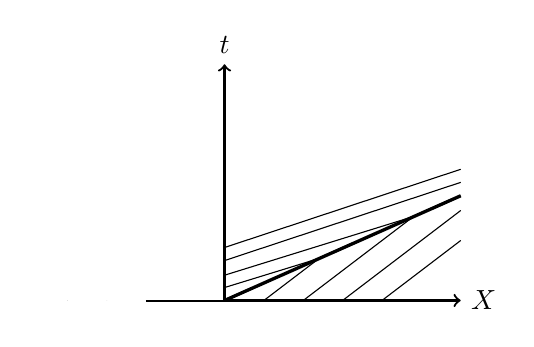
\begin{tikzpicture}
  \draw[->,thick] (-1,0) -- (3,0) node[right] {$X$};
  \draw[->,thick](0,0) -- (0,3) node[above] {$t$};
  \draw(-0.5,0.01) -- (1.20,0.533333) ;
  \draw(-1,0.01) -- (2.40,1.066) ;
  \draw(-1.5,0.01) -- (3,1.5) ;
  \draw(-2,0.01) -- (3,1.666) ;
  %%%%%%%%% 
  \draw(0.5,0) -- (1.20,0.533333) ;
  \draw(1.,0) -- (2.40,1.066) ;
  \draw(1.5,0) -- (3,1.14285) ;
  \draw(2.0,0) -- (3,0.7619) ;
  \draw[very thick] (0,0) -- (3,1.33);
  \fill[white] (-2.5,2.5) rectangle (-0.015,0.01);
  \fill[white] (-2.,0) rectangle (-1.,0.1);
\end{tikzpicture}}
  \subcaptionbox{Right-going simple wave\label{subfig:2R}}{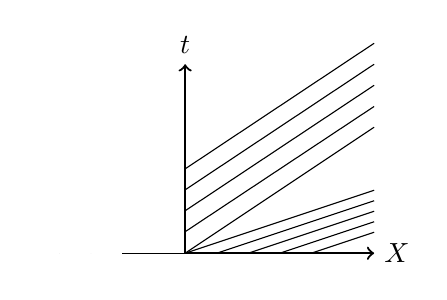
\begin{tikzpicture}[scale=0.8]
  \draw[->,thick] (-1,0) -- (3,0) node[right] {$X$};
  \draw[->,thick](0,0) -- (0,3) node[above] {$t$};
  \draw(0,0) -- (3,2) ;
  \draw(-0.5,0.01) -- (3,2.33) ;
  \draw(-1,0.01) -- (3,2.666) ;
  \draw(-1.5,0.01) -- (3,3) ;
  \draw(-2,0.01) -- (3,3.333) ;
  \draw(0,0) -- (3,1) ;
  \draw(0.5,0) -- (3,0.833) ;
  \draw(1,0) -- (3,0.666) ;
  \draw(1.5,0) -- (3,0.5) ;
  \draw(2,0) -- (3,0.333);
  \fill[white] (-2.5,2.5) rectangle (-0.015,0.01);
  \fill[white] (-2.,0) rectangle (-1.,0.1);
\end{tikzpicture}}
 \caption{Solutions of the Picard problem \eqref{eq:Picard_problem} depending on initial and boundary data.}
  \label{fig:Picard_problem}
\end{figure}

\subsubsection*{Shock waves}
% Applying the method of characteristics between the $x$-axis and an intersection point of two characteristic straight lines, one shows that a shock wave carry a jump discontinuity.
A shock wave is a discontinuous wave hence satisfying the Rankine-Hugoniot condition \eqref{eq:rankine-hugoniot}:
\begin{align}
  \label{eq:RH_velocity}
  & -\frac{1}{\rho_0}\(\bar{\Pi} - \Pi_R \) = s \( \bar{v} - v_R \)\\
  \label{eq:RH_F}
  & - \( \bar{v}-v_R\)=s\( \bar{F} - F_R\)
\end{align}
where the shock speed $s$ is to be defined.
In what follows, $\bar{F}$ is considered as an unknown so that a relation connecting $\Qcb^R$ to a set of solutions $\Qcb$ through a shock wave can be developed.
Substitution of $s$ from equation \eqref{eq:RH_F} and introduction in equation \eqref{eq:RH_velocity} where $\Pi=\frac{\lambda+2\mu}{2}\(F^3-F\)$ yield:
\begin{align}
  \label{eq:shock_speed}
  & s=-\frac{\bar{v}-v_R}{\bar{F} - F_R}\\
  \label{eq:v_jump}
  & \bar{v}-v_R= \pm \sqrt{\frac{\lambda+2\mu}{2\rho_0}(\bar{F}-F_R)\[ \bar{F}^3-\bar{F} - (F_R^3-F_R)\]}
\end{align}
In addition to the Rankine-Hugoniot condition, the \textit{Lax entropy condition} stating that characteristic curves collide in a shock wave must be satisfied \cite[p.268]{Leveque}:
\begin{equation}
  \label{eq:Lax_entropy}
  c(\bar{F})<s<c(F_R)
\end{equation}
For the problem considered here ($\bar{F}>F$), the Lax condition is automatically satisfied. As a consequence, the square root in equation \eqref{eq:v_jump} is real, leading to two families of curves in the phase plane ($F,v$). \thomas{One of those curve is expected to identify with the jump conditions derived for the linear case \eqref{eq:jump_star_R} when considering an infinitesimal jump } (\textit{i.e. $\bar{F}=F_R+\epsilon$ with $\epsilon \rightarrow 0$}). Thus, equation \eqref{eq:v_jump} reads:
\begin{equation}
  \label{eq:linearization}
  \bar{v}-v_R= \pm \sqrt{\frac{\lambda+2\mu}{2\rho_0}\epsilon\[ (F_R+\epsilon)^3-(F_R+\epsilon) - (F_R^3-F_R)\]}
\end{equation}
where, with $\epsilon \rightarrow 0$:
\begin{equation*}
  (F_R+\epsilon)^3\approx F_R^3(1+\frac{3\epsilon}{F_R})
\end{equation*}
so that:
\begin{equation*}
  \matrice{\bar{v} \\ \bar{F}}=\matrice{v_R \\ F_R} + \epsilon \matrice{\pm \sqrt{\frac{\lambda+2\mu}{2\rho_0}\[ 3F_R^2-1\]}\\1}
\end{equation*}
The minus sign allows to recover the right eigenvector associated to the right-going wave and therefore corresponds to a right-going shock wave. On the other hand, the plus sign stands for left-going shocks. Finally, the Rankine-Hugoniot condition across a left-going shock and a right-going shock respectively lead to:
\begin{align}
  \label{eq:left-going_shock}
  &\bar{v}-v_L= \sqrt{\frac{\lambda+2\mu}{2\rho_0}(\bar{F}-F_L)\[ \bar{F}^3-\bar{F} - (F_L^3-F_L)\]} \\
  \label{eq:right-going_shock}
  &\bar{v}-v_R= -\sqrt{\frac{\lambda+2\mu}{2\rho_0}(\bar{F}-F_R)\[ \bar{F}^3-\bar{F} - (F_R^3-F_R)\]}
\end{align}

\subsubsection*{Simple waves}
In order to study the evolution of fields within the region bounded by characteristics that move away in figure \ref{fig:Picard_problem}\subref{subfig:2R}, let's write the left-going characteristic equation through it with $\Lcb^1=[1,-c_1]$:
\begin{equation}
  \label{eq:SVK_rarefaction}
  dv -c_1(F)  dF = 0 
\end{equation}
The complete set of states $\Qcb$ connected to $\Qcb^R$ through a simple wave is obtained by integration of equation \eqref{eq:SVK_rarefaction}. Note that this integration results in a smooth evolution of fields inside a simple wave even for discontinuous initial conditions, unlike shocks. Moreover, the vanishing right-hand side of the conservative form of Picard problem \eqref{eq:Picard_problem} yields a similarity solution. The particular case of simple wave constant along each ray $\xi=x/t$ corresponds to a \textit{rarefaction wave} \cite{Leveque}. 

Integration of equation \eqref{eq:SVK_rarefaction} is performed by using the change of variable: $F \mapsto ch(x)/\sqrt{3}$ so that one gets:
%The following change of variable is then introduced: $F \mapsto ch(x)/\sqrt{3}$, so that  becomes:
\begin{equation}
  \label{eq:charac_equation_sh}
  dv=-\sqrt{\frac{\lambda + 2\mu}{6\rho_0}}sh(x)^2 dx
\end{equation}
where, the hyperbolic cosine $ch(x)$ and sine $sh(x)$ satisfy: $ch(x)^2-sh(x)^2=1$. Equation \eqref{eq:charac_equation_sh} can be easily integrated with the exponential form of hyperbolic sine: $sh(x)=\frac{e^x - e^{-x}}{2}$, thus yielding:
\begin{equation*}
  v-v_R=-\frac{1}{4}\sqrt{\frac{\lambda + 2\mu}{6\rho_0}}\[sh(2x)-2x -(sh(2x_R)-2x_R)\]
\end{equation*}
At last, the inverse change of variable leads to the relation:
\begin{equation}
  \label{eq:integral_curve_right}
  v-v_R=-\sqrt{\frac{\lambda + 2\mu}{24\rho_0}}\[\sqrt{3}\(F\sqrt{3F^2-1} -F_R\sqrt{3F_R^2-1}\)-\ln\(\frac{\sqrt{3}F + \sqrt{3F^2-1}}{\sqrt{3}F_R + \sqrt{3F_R^2-1}}\) \]
\end{equation}
In a similar manner, $dv -c_2(F)  dF = 0$ must hold through a left-going rarefaction wave so that:
\begin{equation}
  \label{eq:integral_curve_left}
  v-v_L=\sqrt{\frac{\lambda + 2\mu}{24\rho_0}}\[\sqrt{3}\(F\sqrt{3F^2-1} -F_L\sqrt{3F_L^2-1}\)-\ln\(\frac{\sqrt{3}F + \sqrt{3F^2-1}}{\sqrt{3}F_L + \sqrt{3F_L^2-1}}\) \]
\end{equation}

Equations \eqref{eq:integral_curve_right} and \eqref{eq:integral_curve_left} correspond to \textit{integral curves} that connect initial conditions to a set of solutions through a right-going or a left-going rarefaction respectively.

\subsubsection*{Solution of the Riemann problem}
The above developments are now generalized by considering the Riemann problem in an infinite medium:
\begin{equation}
  \label{eq:HE_Riemann_problem}
  \begin{aligned}
    &\Qcb_t + \drond{\Fcb\cdot \vect{N}}{X_N} = \vect{0}, \\
    &\left\lbrace 
      \begin{aligned}
        & \Qcb(X_N,t=0) = \Qcb^L = \matrice{v=0 \\ F_L} \quad \text{if } X_N< 0\\
        & \Qcb(X_N,t=0) = \Qcb^R = \matrice{v=0 \\ F_R}\quad \text{if } X_N> 0
      \end{aligned}
    \right.
  \end{aligned}
\end{equation}
such that the plane wave state \eqref{eq:SVK_plane_wave} holds.
As for the Picard problem, initial conditions influence the characteristic structure of the solution. Indeed, if initial conditions are given such that $F_L<F_R$, left-going characteristics will collide while right-going ones will move away from one another (see figure \ref{fig:RP_solution}\subref{subfig:1S2R}). In that case, the first and second characteristic fields are respectively referred to as a \textit{1-shock} and a \textit{2-rarefaction}. Conversely, if $F_L>F_R$ the solution corresponds to a \textit{1-rarefaction} and a \textit{2-shock} (figure \ref{fig:RP_solution}\subref{subfig:1R2S}). 

\begin{figure}[h]
  \centering
  \subcaptionbox{$F_L < F_R$\label{subfig:1S2R}}{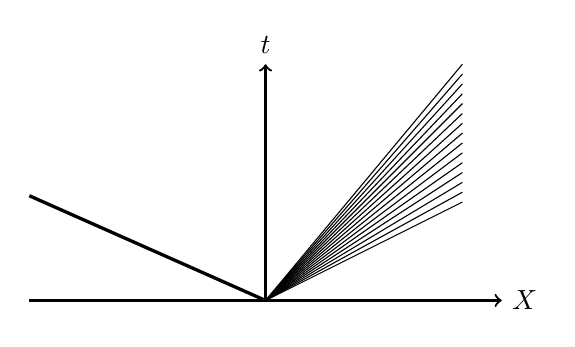
\begin{tikzpicture}
  \draw[->,thick] (-3,0) -- (3,0) node[right] {$X$};
  \draw[->,thick](0,0) -- (0,3) node[above] {$t$};
  %% Shock wave
  \draw[very thick] (0,0) -- (-3,1.33);
  %% Rarefaction wave
  \foreach \x in {0.5,0.55,...,1.25}
  \draw(0,0) -- (2.5,2.5*\x) ;
\end{tikzpicture}}
  \subcaptionbox{$F_L > F_R$\label{subfig:1R2S}}{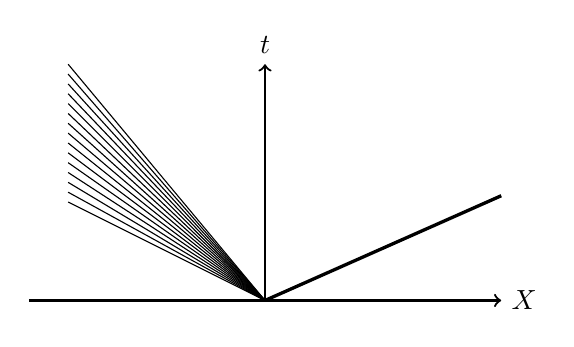
\begin{tikzpicture}
  \draw[->,thick] (-3,0) -- (3,0) node[right] {$X$};
  \draw[->,thick](0,0) -- (0,3) node[above] {$t$};
  %% Shock wave
  \draw[very thick] (0,0) -- (3,1.33);
  %% Rarefaction wave
  \foreach \x in {0.5,0.55,...,1.25}
  \draw(0,0) -- (-2.5,2.5*\x) ;
\end{tikzpicture}}
  \caption{General wave patterns arising in the solution of the Riemann problem \eqref{eq:HE_Riemann_problem} depending on initial data. (a): 1-shock--2-rarefaction. (b): 1-rarefaction--2-shock.}
  \label{fig:RP_solution}
\end{figure}

For the 1-shock--2-rarefaction solution one then seeks a state $\Qcb$ that is connected to $\Qcb^L$ and $\Qcb^R$ through a shock wave and a rarefaction wave respectively. Hence, $\Qcb$ must satisfy equations \eqref{eq:left-going_shock} and \eqref{eq:integral_curve_right}, that is:
\begin{equation}
  \label{eq:1S2R_solution}
  \left\lbrace
  \begin{aligned}
    &v -v_L= \sqrt{\frac{\lambda+2\mu}{2\rho_0}(F -F_L)\[ F^3-F  - (F_L^3-F_L)\]} \\
    &v -v_R=-\sqrt{\frac{\lambda + 2\mu}{24\rho_0}}\[\sqrt{3}\(F \sqrt{3F^2-1} -F_R\sqrt{3F_R^2-1}\)-\ln\(\frac{\sqrt{3}F  + \sqrt{3F^2-1}}{\sqrt{3}F_R + \sqrt{3F_R^2-1}}\) \]
  \end{aligned}
  \right.
\end{equation}
Analogously, the 1-rarefaction--2-shock solution is given by the solution of equations \eqref{eq:integral_curve_left} and \eqref{eq:right-going_shock}:
\begin{equation}
  \label{eq:1R2S_solution}
  \left\lbrace
  \begin{aligned}
    &v -v_L=\sqrt{\frac{\lambda + 2\mu}{24\rho_0}}\[\sqrt{3}\(F \sqrt{3F^2-1} -F_L\sqrt{3F_L^2-1}\)-\ln\(\frac{\sqrt{3}F  + \sqrt{3F^2-1}}{\sqrt{3}F_L + \sqrt{3F_L^2-1}}\) \]\\
    &v -v_R= -\sqrt{\frac{\lambda+2\mu}{2\rho_0}(F -F_R)\[ F^3-F  - (F_R^3-F_R)\]}
  \end{aligned}
  \right.
\end{equation}
\begin{figure}[h!]
  \centering
  {\definecolor{Purple}{RGB}{120,28,129}
\definecolor{Blue}{RGB}{63,96,174}
\definecolor{Duck}{RGB}{83,158,182}
\definecolor{Green}{RGB}{109,179,136}
\definecolor{Yellow}{RGB}{202,184,67}
\definecolor{Orange}{RGB}{231,133,50}
\definecolor{Red}{RGB}{217,33,32}
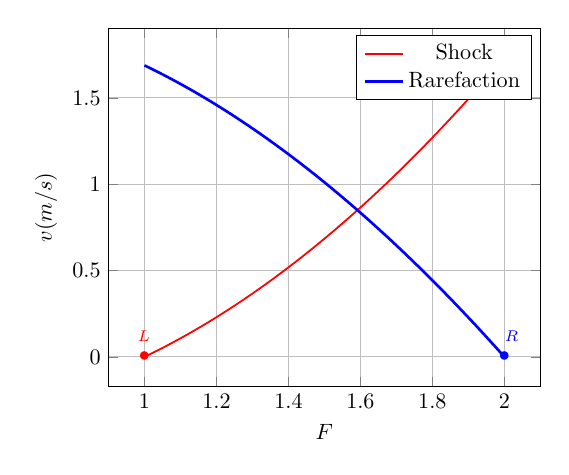
\begin{tikzpicture}[scale=0.8]
\begin{axis}[xlabel=$F$,ylabel=$v (m/s)$,ymajorgrids=true,xmajorgrids=true]
  \addplot[Red,thick] coordinates {(1.0,0.0) (1.0196019601960196,0.019889905868838792) (1.0392039203920391,0.04035480171519238) (1.058805880588059,0.06139339246981025) (1.0784078407840785,0.08300445472552491) (1.098009800980098,0.1051868317293367) (1.1176117611761176,0.1279394287977403) (1.1372137213721372,0.1512612091133456) (1.1568156815681567,0.17515118986560513) (1.1764176417641765,0.19960843870261852) (1.196019601960196,0.2246320704646163) (1.2156215621562156,0.25022124417291264) (1.2352235223522352,0.2763751602509047) (1.2548254825482548,0.30309305795616337) (1.2744274427442743,0.330374213004825) (1.2940294029402941,0.3582179353714115) (1.3136313631363137,0.386623567248899) (1.3332333233323332,0.4155904811553686) (1.3528352835283528,0.445118078174895) (1.3724372437243724,0.47520578632153143) (1.3920392039203922,0.5058530590163028) (1.4116411641164117,0.5370593736680643) (1.4312431243124313,0.568824230349938) (1.4508450845084508,0.6011471505637854) (1.4704470447044704,0.6340276760858663) (1.4900490049004902,0.667465367887438) (1.5096509650965095,0.7014598051246006) (1.5292529252925293,0.7360105841921958) (1.5488548854885489,0.7711173178369951) (1.5684568456845684,0.8067796343258441) (1.5880588058805882,0.8429971766647708) (1.6076607660766076,0.8797696018654025) (1.6272627262726274,0.917096580255355) (1.646864686468647,0.9549777948294852) (1.6664666466646665,0.9934129406392047) (1.686068606860686,1.032401724217221) (1.7056705670567056,1.0719438630353144) (1.7252725272527254,1.1120390849929296) (1.7448744874487447,1.1526871279345328) (1.7644764476447645,1.1938877391938512) (1.784078407840784,1.2356406751632294) (1.8036803680368036,1.2779457008865038) (1.8232823282328234,1.320802589673878) (1.8428842884288428,1.3642111227374165) (1.8624862486248626,1.4081710888458763) (1.8820882088208821,1.4526822839976499) (1.9016901690169017,1.4977445111107466) (1.9212921292129215,1.543357579728744) (1.9408940894089408,1.5895213057417645) (1.9604960496049606,1.6362355111215798) (1.9800980098009802,1.6835000236699957) (1.9996999699969997,1.7313146767797576) };
  \addplot[Blue,very thick] coordinates {(1.0,1.6884673989302577) (1.0196019601960196,1.6685781823289632) (1.0392039203920391,1.648117983645035) (1.058805880588059,1.6270917763366024) (1.0784078407840785,1.6055041425368688) (1.098009800980098,1.5833593157699348) (1.1176117611761176,1.5606612177002648) (1.1372137213721372,1.5374134899261505) (1.1568156815681567,1.5136195216278194) (1.1764176417641765,1.48928247372591) (1.196019601960196,1.4644053000848238) (1.2156215621562156,1.4389907661996928) (1.2352235223522352,1.4130414657294894) (1.2548254825482548,1.3865598351776642) (1.2744274427442743,1.3595481669723095) (1.2940294029402941,1.3320086211576845) (1.3136313631363137,1.3039432358761032) (1.3332333233323332,1.2753539367920979) (1.3528352835283528,1.246242545588463) (1.3724372437243724,1.216610787645106) (1.3920392039203922,1.1864602989961286) (1.4116411641164117,1.1557926326474621) (1.4312431243124313,1.12460926432638) (1.4508450845084508,1.092911597724879) (1.4704470447044704,1.0607009692909792) (1.4900490049004902,1.0279786526152188) (1.5096509650965095,0.994745862453826) (1.5292529252925293,0.9610037584250569) (1.5488548854885489,0.9267534484108921) (1.5684568456845684,0.8919959916925568) (1.5880588058805882,0.8567324018451127) (1.6076607660766076,0.8209636494135533) (1.6272627262726274,0.7846906643903794) (1.646864686468647,0.7479143385125069) (1.6664666466646665,0.7106355273934435) (1.686068606860686,0.6728550525050632) (1.7056705670567056,0.6345737030218022) (1.7252725272527254,0.595792237538853) (1.7448744874487447,0.5565113856747698) (1.7644764476447645,0.5167318495678894) (1.784078407840784,0.47645430527509447) (1.8036803680368036,0.43567940408061234) (1.8232823282328234,0.3944077737218566) (1.8428842884288428,0.3526400195386741) (1.8624862486248626,0.31037672555176576) (1.8820882088208821,0.2676184554755838) (1.9016901690169017,0.22436575367049583) (1.9212921292129215,0.18061914603862234) (1.9408940894089408,0.13637914086738703) (1.9604960496049606,0.09164622962443836) (1.9800980098009802,0.04642088770736517) (1.9996999699969997,0.0007035751512764867) };
  \node at (axis cs:1,0) [Red] {$\bullet$};
  \node at (axis cs:2.,0) [Blue] {$\bullet$};
  % \node[coordinate] at (axis cs:1.,0.) {$Mich$};
  \node at (axis cs:1,0) [anchor=south,Red] {$\Qcb^L$};
  \node at (axis cs:1.98,0) [above right,Blue] {$\Qcb^R$};
  \legend{Shock,Rarefaction}
  % \addplot[Blue,dashed,very thick,domain=1:2,samples=51,samples y=0]
  %   ({x},{0.-sqrt(0.5*(12.-1))*(x-2.)});
  % \addplot[Red,dashed,very thick,domain=1:2,samples=51,samples y=0]
  %   ({x},{0.+sqrt(0.5*(2.-1))*(x-1.)});
\end{axis}
\end{tikzpicture}
\phantomsubcaption \label{subfig:1S2R_curves}}
  {\definecolor{Purple}{RGB}{120,28,129}
\definecolor{Blue}{RGB}{63,96,174}
\definecolor{Duck}{RGB}{83,158,182}
\definecolor{Green}{RGB}{109,179,136}
\definecolor{Yellow}{RGB}{202,184,67}
\definecolor{Orange}{RGB}{231,133,50}
\definecolor{Red}{RGB}{217,33,32}
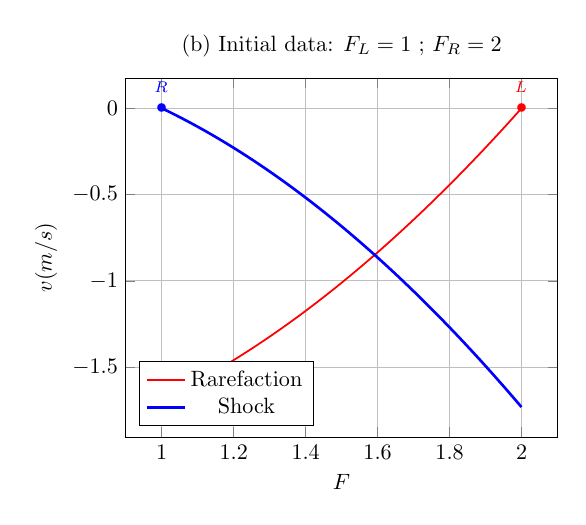
\begin{tikzpicture}[scale=0.8]
\begin{axis}[xlabel=$F$,ylabel=$v (m/s)$,ymajorgrids=true,xmajorgrids=true,legend pos=south west,title={(b) Initial data: $F_L=1$ ; $F_R=2$}]
  \addplot[Red,thick] coordinates {(1.0,-1.6884673989302577) (1.0196019601960196,-1.6685781823289632) (1.0392039203920391,-1.648117983645035) (1.058805880588059,-1.6270917763366024) (1.0784078407840785,-1.6055041425368688) (1.098009800980098,-1.5833593157699348) (1.1176117611761176,-1.5606612177002648) (1.1372137213721372,-1.5374134899261505) (1.1568156815681567,-1.5136195216278194) (1.1764176417641765,-1.48928247372591) (1.196019601960196,-1.4644053000848238) (1.2156215621562156,-1.4389907661996928) (1.2352235223522352,-1.4130414657294894) (1.2548254825482548,-1.3865598351776642) (1.2744274427442743,-1.3595481669723095) (1.2940294029402941,-1.3320086211576845) (1.3136313631363137,-1.3039432358761032) (1.3332333233323332,-1.2753539367920979) (1.3528352835283528,-1.246242545588463) (1.3724372437243724,-1.216610787645106) (1.3920392039203922,-1.1864602989961286) (1.4116411641164117,-1.1557926326474621) (1.4312431243124313,-1.12460926432638) (1.4508450845084508,-1.092911597724879) (1.4704470447044704,-1.0607009692909792) (1.4900490049004902,-1.0279786526152188) (1.5096509650965095,-0.994745862453826) (1.5292529252925293,-0.9610037584250569) (1.5488548854885489,-0.9267534484108921) (1.5684568456845684,-0.8919959916925568) (1.5880588058805882,-0.8567324018451127) (1.6076607660766076,-0.8209636494135533) (1.6272627262726274,-0.7846906643903794) (1.646864686468647,-0.7479143385125069) (1.6664666466646665,-0.7106355273934435) (1.686068606860686,-0.6728550525050632) (1.7056705670567056,-0.6345737030218022) (1.7252725272527254,-0.595792237538853) (1.7448744874487447,-0.5565113856747698) (1.7644764476447645,-0.5167318495678894) (1.784078407840784,-0.47645430527509447) (1.8036803680368036,-0.43567940408061234) (1.8232823282328234,-0.3944077737218566) (1.8428842884288428,-0.3526400195386741) (1.8624862486248626,-0.31037672555176576) (1.8820882088208821,-0.2676184554755838) (1.9016901690169017,-0.22436575367049583) (1.9212921292129215,-0.18061914603862234) (1.9408940894089408,-0.13637914086738703) (1.9604960496049606,-0.09164622962443836) (1.9800980098009802,-0.04642088770736517) (1.9996999699969997,-0.0007035751512764867) };
  \addplot[Blue,very thick] coordinates {(1.0,0.0) (1.0196019601960196,-0.019889905868838792) (1.0392039203920391,-0.04035480171519238) (1.058805880588059,-0.06139339246981025) (1.0784078407840785,-0.08300445472552491) (1.098009800980098,-0.1051868317293367) (1.1176117611761176,-0.1279394287977403) (1.1372137213721372,-0.1512612091133456) (1.1568156815681567,-0.17515118986560513) (1.1764176417641765,-0.19960843870261852) (1.196019601960196,-0.2246320704646163) (1.2156215621562156,-0.25022124417291264) (1.2352235223522352,-0.2763751602509047) (1.2548254825482548,-0.30309305795616337) (1.2744274427442743,-0.330374213004825) (1.2940294029402941,-0.3582179353714115) (1.3136313631363137,-0.386623567248899) (1.3332333233323332,-0.4155904811553686) (1.3528352835283528,-0.445118078174895) (1.3724372437243724,-0.47520578632153143) (1.3920392039203922,-0.5058530590163028) (1.4116411641164117,-0.5370593736680643) (1.4312431243124313,-0.568824230349938) (1.4508450845084508,-0.6011471505637854) (1.4704470447044704,-0.6340276760858663) (1.4900490049004902,-0.667465367887438) (1.5096509650965095,-0.7014598051246006) (1.5292529252925293,-0.7360105841921958) (1.5488548854885489,-0.7711173178369951) (1.5684568456845684,-0.8067796343258441) (1.5880588058805882,-0.8429971766647708) (1.6076607660766076,-0.8797696018654025) (1.6272627262726274,-0.917096580255355) (1.646864686468647,-0.9549777948294852) (1.6664666466646665,-0.9934129406392047) (1.686068606860686,-1.032401724217221) (1.7056705670567056,-1.0719438630353144) (1.7252725272527254,-1.1120390849929296) (1.7448744874487447,-1.1526871279345328) (1.7644764476447645,-1.1938877391938512) (1.784078407840784,-1.2356406751632294) (1.8036803680368036,-1.2779457008865038) (1.8232823282328234,-1.320802589673878) (1.8428842884288428,-1.3642111227374165) (1.8624862486248626,-1.4081710888458763) (1.8820882088208821,-1.4526822839976499) (1.9016901690169017,-1.4977445111107466) (1.9212921292129215,-1.543357579728744) (1.9408940894089408,-1.5895213057417645) (1.9604960496049606,-1.6362355111215798) (1.9800980098009802,-1.6835000236699957) (1.9996999699969997,-1.7313146767797576) };
  \node at (axis cs:1,0) [Blue] {$\bullet$};
  \node at (axis cs:2.,0) [Red] {$\bullet$};
  \node at (axis cs:1,0) [anchor=south,Blue] {$\Qcb^R$};
  \node at (axis cs:2,0) [anchor=south,Red] {$\Qcb^L$};
\legend{Rarefaction,Shock}
\end{axis}
\end{tikzpicture}
\phantomsubcaption  \label{subfig:1R2S_curves}}
  \caption{Set of connected states $\Qcb$ to initial data through shock and rarefaction waves with $v_L=v_R=0$ in both cases: (a) 1-shock, 2-rarefaction solution ; (b) 1-rarefaction, 2-shock.}
  \label{fig:solutions_RP}
\end{figure} 
Once one of this system is solved, the solution $\Qcb$ is known everywhere except inside the rarefaction fan. Nevertheless, in this region $\Qcb$ only varies with the ray $\xi=c_i(F)$ and hence, the solution inside an $i$-rarefaction wave satisfies:
\begin{equation}
  \label{eq:rarefaction_fan}
  \xi = \pm \sqrt{\frac{\lambda + 2\mu}{2\rho_0}\(3F^2-1 \)} \quad \Rightarrow \quad F(\xi)= \sqrt{\frac{2\rho_0}{3(\lambda + 2\mu)}\xi^2-1}
\end{equation}

The curves corresponding to equations \eqref{eq:1S2R_solution} and \eqref{eq:1R2S_solution} are depicted in figures \ref{fig:solutions_RP}\subref{subfig:1S2R_curves} and \ref{fig:solutions_RP}\subref{subfig:1R2S_curves} for parameter values such that $\frac{\lambda+2\mu}{\rho_0}=1$. In both cases, the solution $\Qcb(x,t)$ in the region bounded by the shock and the rarefaction fan is given by the intersection of curves in the phase plane. 

\begin{remark}
  Note that the above developments are based on a constitutive model that leads to a concave flux function $\Fcb^T=-\[\frac{1}{\rho_0}\Pi \: ;\: v\]$ (\textit{i.e. } $\ddrond{\Pi}{F}{F}>0$). As a consequence, the characteristic speeds are monotonically increasing functions of the deformation gradient (in absolute value). Since the dependence of characteristic speeds on the deformation gradient governs the wave pattern (\textit{i.e.: either a rarefaction or a shock wave}), the structure of the solution differs from other constitutive laws with convex flux function such as the neo-Hookean model.
  Comparisons of ($F,\Pi_{11}$) and ($F,\abs{c}$) are shown in figures \ref{fig:SVK-NH}\subref{subfig:SVK_NH_Pi} and \ref{fig:SVK-NH}\subref{subfig:SVK_NH_speeds} as an illustration of previous remarks.
  \begin{figure}[h!]
    \centering
    {\definecolor{Red}{RGB}{217,33,32}
\definecolor{Blue}{RGB}{63,96,174}
\definecolor{Duck}{RGB}{83,158,182}
\definecolor{Green}{RGB}{109,179,136}
\definecolor{Yellow}{RGB}{202,184,67}
\definecolor{Orange}{RGB}{231,133,50}
\definecolor{Red}{RGB}{217,33,32}
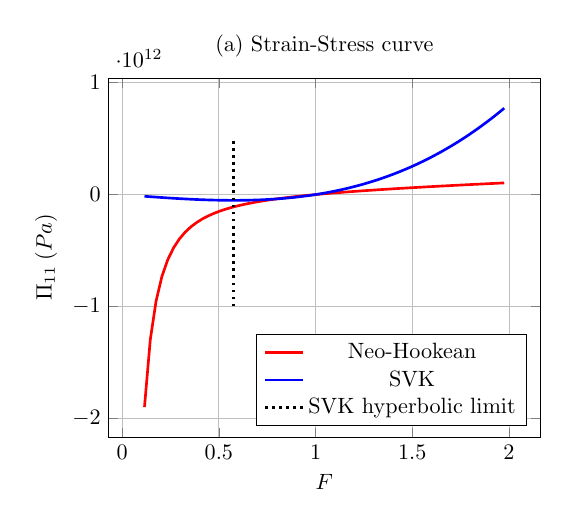
\begin{tikzpicture}[scale=0.8]
\begin{axis}[xlabel=$F$,ylabel=$\Pi_{11} \: (Pa)$,ymajorgrids=true,xmajorgrids=true,legend pos=south east,title={(a) Strain-Stress curve}]
\addplot[Red,very thick] coordinates {(0.11547005383792518,-1898966453319.162) (0.14547005383792516,-1296837707486.0405) (0.17547005383792513,-951312235719.5623) (0.20547005383792513,-732355105152.6451) (0.23547005383792513,-583575852118.2125) (0.2654700538379251,-477087968993.8754) (0.2954700538379251,-397729449724.4541) (0.3254700538379251,-336642141070.28204) (0.35547005383792507,-288349957545.72546) (0.38547005383792504,-249309520683.61847) (0.415470053837925,-217140040714.9308) (0.44547005383792504,-190190468824.5224) (0.475470053837925,-167284549773.97247) (0.505470053837925,-147564580724.34894) (0.535470053837925,-130392343185.27245) (0.5654700538379249,-115284401045.16144) (0.595470053837925,-101868733030.67676) (0.625470053837925,-89854990617.66492) (0.6554700538379249,-79013679521.07468) (0.6854700538379249,-69161318053.14328) (0.7154700538379248,-60149680216.69014) (0.7454700538379249,-51857881714.88495) (0.7754700538379249,-44186477584.150566) (0.8054700538379248,-37053004869.531456) (0.8354700538379248,-30388577783.986546) (0.8654700538379249,-24135259235.847366) (0.8954700538379248,-18244011798.887867) (0.9254700538379248,-12673085866.843775) (0.9554700538379248,-7386740998.494719) (0.9854700538379247,-2354223588.251995) (1.0154700538379247,2451056537.9352818) (1.0454700538379247,7052193879.264957) (1.0754700538379247,11469332294.041113) (1.1054700538379247,15720112571.176903) (1.1354700538379248,19820042073.450085) (1.1654700538379246,23782801671.8228) (1.1954700538379246,27620501912.14364) (1.2254700538379246,31343897846.142628) (1.2554700538379246,34962570023.63762) (1.2854700538379247,38485077640.53793) (1.3154700538379245,41919088663.206696) (1.3454700538379245,45271490826.59238) (1.3754700538379245,48548486673.378265) (1.4054700538379246,51755675220.64049) (1.4354700538379246,54898122376.10795) (1.4654700538379246,57980421852.87309) (1.4954700538379244,61006748029.95563) (1.5254700538379244,63980901961.52675) (1.5554700538379245,66906351538.24785) (1.5854700538379245,69786266641.0072) (1.6154700538379245,72623549993.23035) (1.6454700538379243,75420864307.28705) (1.6754700538379244,78180656228.87244) (1.7054700538379244,80905177507.05946) (1.7354700538379244,83596503754.174) (1.7654700538379244,86256551106.45828) (1.7954700538379245,88887091051.8295) (1.8254700538379243,91489763653.42323) (1.8554700538379243,94066089365.83081) (1.8854700538379243,96617479614.0105) (1.9154700538379243,99145246281.97147) (1.9454700538379244,101650610238.83322) (1.9754700538379242,104134709013.2085) };
\addplot[Blue,very thick] coordinates {(0.11547005383792518,-15336791766.165447) (0.14547005383792516,-19168111304.289738) (0.17547005383792513,-22893685303.277996) (0.20547005383792513,-26491706070.822536) (0.23547005383792513,-29940365914.61566) (0.2654700538379251,-33217857142.349674) (0.2954700538379251,-36302372061.71689) (0.3254700538379251,-39172102980.40962) (0.35547005383792507,-41805242206.12016) (0.38547005383792504,-44179982046.540825) (0.415470053837925,-46274514809.36392) (0.44547005383792504,-48067032802.28176) (0.475470053837925,-49535728332.98665) (0.505470053837925,-50658793709.17089) (0.535470053837925,-51414421238.526794) (0.5654700538379249,-51780803228.74666) (0.595470053837925,-51736131987.522804) (0.625470053837925,-51258599822.54755) (0.6554700538379249,-50326399041.513176) (0.6854700538379249,-48917721952.112) (0.7154700538379248,-47010760862.036354) (0.7454700538379249,-44583708078.97849) (0.7754700538379249,-41614755910.630775) (0.8054700538379248,-38082096664.68549) (0.8354700538379248,-33963922648.83495) (0.8654700538379249,-29238426170.77144) (0.8954700538379248,-23883799538.187305) (0.9254700538379248,-17878235058.774815) (0.9554700538379248,-11199925040.226295) (0.9854700538379247,-3827061790.2340784) (1.0154700538379247,4262162383.5095387) (1.0454700538379247,13089555173.312326) (1.0754700538379247,22676924271.481888) (1.1054700538379247,33046077370.32594) (1.1354700538379248,44218822162.15218) (1.1654700538379246,56216966339.268196) (1.1954700538379246,69062317593.98189) (1.2254700538379246,82776683618.60081) (1.2554700538379246,97381872105.43274) (1.2854700538379247,112899690746.78526) (1.3154700538379245,129351947234.96603) (1.3454700538379245,146760449262.28293) (1.3754700538379245,165147004521.04358) (1.4054700538379246,184533420703.55563) (1.4354700538379246,204941505502.12674) (1.4654700538379246,226393066609.06476) (1.4954700538379244,248909911716.677) (1.5254700538379244,272513848517.2716) (1.5554700538379245,297226684703.1562) (1.5854700538379245,323070227966.6382) (1.6154700538379245,350066286000.0256) (1.6454700538379243,378236666495.6256) (1.6754700538379244,407603177145.7466) (1.7054700538379244,438187625642.6959) (1.7354700538379244,470011819678.7812) (1.7654700538379244,503097566946.3102) (1.7954700538379245,537466675137.5906) (1.8254700538379243,573140951944.9299) (1.8554700538379243,610142205060.6364) (1.8854700538379243,648492242177.0171) (1.9154700538379243,688212870986.3801) (1.9454700538379244,729325899181.0331) (1.9754700538379242,771853134453.2832) };
\addplot[dotted,very thick] coordinates {(sqrt(1./3.),-1.e12) (sqrt(1./3.),0.5e12)};
\legend{Neo-Hookean,SVK,SVK hyperbolic limit}
\end{axis}
\end{tikzpicture}
 \phantomsubcaption \label{subfig:SVK_NH_Pi}}
    {\definecolor{Red}{RGB}{217,33,32}
\definecolor{Blue}{RGB}{63,96,174}
\definecolor{Duck}{RGB}{83,158,182}
\definecolor{Green}{RGB}{109,179,136}
\definecolor{Yellow}{RGB}{202,184,67}
\definecolor{Orange}{RGB}{231,133,50}
\definecolor{Red}{RGB}{217,33,32}
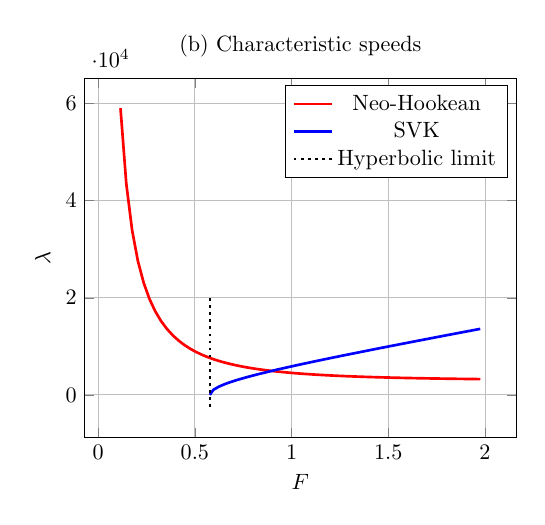
\begin{tikzpicture}[scale=0.8]
\begin{axis}[xlabel=$F$,ylabel=$\abs{\lambda}$,ymajorgrids=true,xmajorgrids=true,title={(b) Characteristic speeds}]
\addplot[Red,very thick] coordinates {(0.11547005383792518,59012.035730808406) (0.14547005383792516,43444.15680640866) (0.17547005383792513,33909.66271892359) (0.20547005383792513,27551.616086072518) (0.23547005383792513,23052.45426344622) (0.2654700538379251,19726.297080765253) (0.2954700538379251,17183.410876622853) (0.3254700538379251,15187.108927674422) (0.35547005383792507,13585.92851121213) (0.38547005383792504,12278.756336822797) (0.415470053837925,11195.691489974464) (0.44547005383792504,10286.970773511453) (0.475470053837925,9516.269220270638) (0.505470053837925,8856.492138358943) (0.535470053837925,8287.045413546242) (0.5654700538379249,7792.014425579814) (0.595470053837925,7358.918900548452) (0.625470053837925,6977.8428382999955) (0.6554700538379249,6640.81463208358) (0.6854700538379249,6341.3576871839605) (0.7154700538379248,6074.159484360366) (0.7454700538379249,5834.824367261866) (0.7754700538379249,5619.6864514897625) (0.8054700538379248,5425.666332338412) (0.8354700538379248,5250.16012367266) (0.8654700538379249,5090.952654625974) (0.8954700538379248,4946.148920983796) (0.9254700538379248,4814.119475233549) (0.9554700538379248,4693.456563660641) (0.9854700538379247,4582.938625301644) (1.0154700538379247,4481.501352586511) (1.0454700538379247,4388.21394243672) (1.0754700538379247,4302.259484218307) (1.1054700538379247,4222.918668359039) (1.1354700538379248,4149.556178447647) (1.1654700538379246,4081.609265724866) (1.1954700538379246,4018.57810915085) (1.2254700538379246,3960.0176447237714) (1.2554700538379246,3905.530610294456) (1.2854700538379247,3854.761601089376) (1.3154700538379245,3807.391969723345) (1.3454700538379245,3763.135435049281) (1.3754700538379245,3721.7342885593334) (1.4054700538379246,3682.9561065868374) (1.4354700538379246,3646.590892305437) (1.4654700538379246,3612.448584281259) (1.4954700538379244,3580.3568787248346) (1.5254700538379244,3550.1593210921387) (1.5554700538379245,3521.7136296737963) (1.5854700538379245,3494.8902195829423) (1.6154700538379245,3469.5709003379666) (1.6454700538379243,3445.6477242208375) (1.6754700538379244,3423.021965921998) (1.7054700538379244,3401.6032167766175) (1.7354700538379244,3381.308579249105) (1.7654700538379244,3362.061949309672) (1.7954700538379245,3343.793376030597) (1.8254700538379243,3326.438489161275) (1.8554700538379243,3309.9379866615427) (1.8854700538379243,3294.237175216221) (1.9154700538379243,3279.2855576483526) (1.9454700538379244,3265.0364619174256) (1.9754700538379242,3251.446707051308) };
\addplot[Blue,very thick] coordinates {(sqrt(1./3.),0.) (0.595470053837925,1048.9455179543422) (0.625470053837925,1731.1029259571128) (0.6554700538379249,2233.012146664284) (0.6854700538379249,2658.790029377158) (0.7154700538379248,3040.5889001561395) (0.7454700538379249,3393.286396027051) (0.7754700538379249,3725.1576526965905) (0.8054700538379248,4041.336632315833) (0.8354700538379248,4345.250197655363) (0.8654700538379249,4639.309436869055) (0.8954700538379248,4925.279696432755) (0.9254700538379248,5204.494537554574) (0.9554700538379248,5477.987035494905) (0.9854700538379247,5746.574266198714) (1.0154700538379247,6010.9138156437175) (1.0454700538379247,6271.542813975518) (1.0754700538379247,6528.905643538706) (1.1054700538379247,6783.374072186155) (1.1354700538379248,7035.262182069363) (1.1654700538379246,7284.837637447764) (1.1954700538379246,7532.330323596269) (1.2254700538379246,7777.939063134427) (1.2554700538379246,8021.836903239133) (1.2854700538379247,8264.175324905573) (1.3154700538379245,8505.087628335128) (1.3454700538379245,8744.691681060722) (1.3754700538379245,8983.092167747032) (1.4054700538379246,9220.382446402957) (1.4354700538379246,9456.646090866763) (1.4654700538379246,9691.958181097758) (1.4954700538379244,9926.386389147965) (1.5254700538379244,10159.991898394823) (1.5554700538379245,10392.830185782268) (1.5854700538379245,10624.951690800193) (1.6154700538379245,10856.402390269113) (1.6454700538379243,11087.224294354115) (1.6754700538379244,11317.455876364773) (1.7054700538379244,11547.132446624275) (1.7354700538379244,11776.286478876727) (1.7654700538379244,12004.947896244235) (1.7954700538379245,12233.144322567889) (1.8254700538379243,12460.901304010209) (1.8554700538379243,12688.242505014787) (1.8854700538379243,12915.189882077482) (1.9154700538379243,13141.763838254037) (1.9454700538379244,13367.983360890252) (1.9754700538379242,13593.866144695845) };
\addplot[dotted,very thick] coordinates {(sqrt(1./3.),-0.25e4) (sqrt(1./3.),2.e4)};
\legend{Neo-Hookean,SVK,Hyperbolic limit}
\end{axis}
\end{tikzpicture}
 \phantomsubcaption \label{subfig:SVK_NH_speeds}}
    \caption{Comparison of neo-Hookean and Saint-Venant-Kirchhoff hyperelastic models.}
    \label{fig:SVK-NH}
  \end{figure}
  At last, figure \ref{fig:SVK-NH}\subref{subfig:SVK_NH_Pi} shows the non-physical behavior of Saint-Venant-Kirchhoff model for high compression loads that lead to a stress tensor tending to zero.
\end{remark}


%%% Local Variables:
%%% mode: latex
%%% TeX-master: "../mainManuscript"
%%% End: